\documentclass{beamer}
\usepackage{siunitx}
\usepackage{tfrupee}
\let\vec\mathbf
\mode<presentation>
\usepackage{amsmath}
\usepackage{amssymb}
%\usepackage{advdate}
\usepackage{adjustbox}
%\usepackage{subcaption}
\usepackage{enumitem}
\usepackage{multicol}
\usepackage{mathtools}
\usepackage{listings}
\usepackage{url}
\usetheme{Boadilla}
\usecolortheme{lily}
\setbeamertemplate{footline}
{
  \leavevmode%
  \hbox{%
  \begin{beamercolorbox}[wd=\paperwidth,ht=2.25ex,dp=1ex,right]{author in head/foot}%
    \insertframenumber{} / \inserttotalframenumber\hspace*{2ex} 
  \end{beamercolorbox}}%
  \vskip0pt%
}
\setbeamertemplate{navigation symbols}{}
\providecommand{\nCr}[2]{\,^{#1}C_{#2}} % nCr
\providecommand{\nPr}[2]{\,^{#1}P_{#2}} % nPr
\providecommand{\mbf}{\mathbf}
\providecommand{\pr}[1]{\ensuremath{\Pr\left(#1\right)}}
\providecommand{\qfunc}[1]{\ensuremath{Q\left(#1\right)}}
\providecommand{\sbrak}[1]{\ensuremath{{}\left[#1\right]}}
\providecommand{\lsbrak}[1]{\ensuremath{{}\left[#1\right.}}
\providecommand{\rsbrak}[1]{\ensuremath{{}\left.#1\right]}}
\providecommand{\brak}[1]{\ensuremath{\left(#1\right)}}
\providecommand{\lbrak}[1]{\ensuremath{\left(#1\right.}}
\providecommand{\rbrak}[1]{\ensuremath{\left.#1\right)}}
\providecommand{\cbrak}[1]{\ensuremath{\left\{#1\right\}}}
\providecommand{\lcbrak}[1]{\ensuremath{\left\{#1\right.}}
\providecommand{\rcbrak}[1]{\ensuremath{\left.#1\right\}}}
\theoremstyle{remark}
\newtheorem{rem}{Remark}
\newcommand{\sgn}{\mathop{\mathrm{sgn}}}

\providecommand{\res}[1]{\Res\displaylimits_{#1}} 
\providecommand{\norm}[1]{\left\lVert#1\right\rVert}
\providecommand{\mtx}[1]{\mathbf{#1}}
\providecommand{\abs}[1]{\left\vert#1\right\vert}
\providecommand{\fourier}{\overset{\mathcal{F}}{ \rightleftharpoons}}
%\providecommand{\hilbert}{\overset{\mathcal{H}}{ \rightleftharpoons}}
\providecommand{\system}{\overset{\mathcal{H}}{ \longleftrightarrow}}
	%\newcommand{\solution}[2]{\textbf{Solution:}{#1}}
%\newcommand{\solution}{\noindent \textbf{Solution: }}align
\providecommand{\dec}[2]{\ensuremath{\overset{#1}{\underset{#2}{\gtrless}}}}
\newcommand{\myvec}[1]{\ensuremath{\begin{pmatrix}#1\end{pmatrix}}}

\title{Matrices in Geometry - 9.5.1}
\author{EE25BTECH11037  Divyansh}
\date{Sept, 2025}

\begin{document}

\maketitle


\section{Problem}
\begin{frame}
\frametitle{Problem Statement}
Find the roots of 
\begin{align}
    x^2 + 3x -10=0
\end{align}
\end{frame}

\section{Solution}
\begin{frame}{Solution}
Expressing the given equation as parabola 
\begin{align}
    y=x^2 + 3x -10
\end{align}
Representing this equation as a conic section
\begin{align}
    \vec{x}^{\top}\vec{V}\vec{x} + 2\vec{u}^{\top}\vec{x} + f=0 \ , \  \vec{V}=\myvec{1 & 0\\0&0} \ , \  \vec{u}=\myvec{3/2 \\ -1/2} \ ,\ f=-10
\end{align}
We need to find intersection points with $y=0$, that is, the X-axis.
\begin{align}
    \vec{x}=\vec{h} + k \vec{m} \ , \ \vec{h}=\myvec{0 \\ 0} \ , \ \vec{m}=\myvec{1 \\ 0}
\end{align}
\end{frame}

\begin{frame}{Solution}
Substituting $\vec{x} = k \vec{m}$ 
\begin{align}
    k^2\vec{m}^{\top}\vec{V}\vec{m} + 2k\vec{u}^{\top}\vec{m} + f=0 \\
    \implies k= \dfrac{1}{2} \sbrak{ -2\vec{u}^{\top}\vec{m} \ \pm \ \sqrt{4\brak{\vec{u}^{\top}\vec{m}}^2 - 4 f \vec{m}^{\top}\vec{V}\vec{m}}}\\
    \implies k= -\vec{u}^{\top}\vec{m} \ \pm \ \sqrt{\brak{\vec{u}^{\top}\vec{m}}^2-f \vec{m}^{\top}\vec{V}\vec{m}}\\
    \vec{u}^{\top}\vec{m} = \myvec{3/2 & -1/2}\myvec{1 \\0} =3/2 \\
    \vec{m}^{\top}\vec{V}\vec{m}=\myvec{1 & 0}\myvec{1 & 0\\0&0}\myvec{1 \\ 0} = 1\\
    k= -\dfrac{3}{2} \ \pm \ \sqrt{ \dfrac{9}{4 } - \brak{-10} 1} = -\dfrac{3}{2} \ \pm \sqrt{\dfrac{49}{4}}\\
    \implies k= - \dfrac{3}{2} \ \pm \dfrac{7}{2}\implies \boxed{ k= 2 \text{ OR } k=-5}
\end{align}
\end{frame}

\begin{frame}{Solution}
Substituting $k$ into $\vec{x}$, we get
\begin{align}
    \vec{x} = \myvec{2 \\ 0} \text{ OR } \vec{x}=\myvec{-5 \\ 0}
\end{align}
This implies that the roots of $x^2 +3x -10 =0$ are $2$ and $-5$.
\end{frame}
\begin{frame}{Solution}
    \begin{figure}[H]
        \centering
        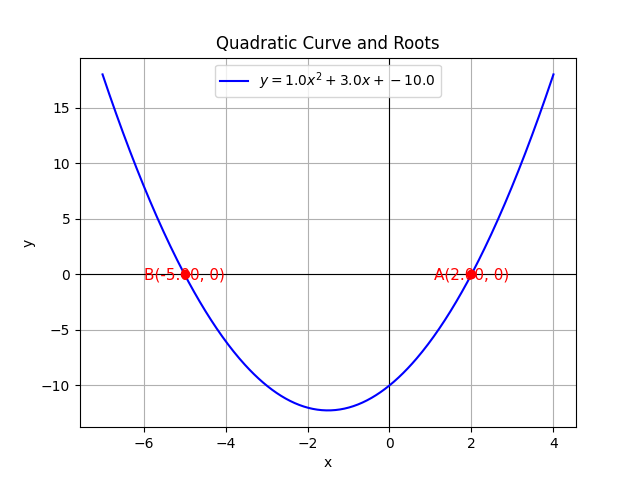
\includegraphics[width=0.5\columnwidth]{figs/1.png}
        \caption{Graph for 9.5.1}
        \label{fig:placeholder}
    \end{figure}
\end{frame}

\end{document}
